As discussed earlier, we propose a solution relying on structural aggregation for visual provenance analysis. This solution follows the pipeline shown in Figure~\ref{fig:overview}, briefly described below.  
%{\color{Fuchsia}As discussed earlier, we propose an instance of our framework \framework{} that is meant to explore provenance traces.
%Our instance leverages a novel solution structural aggregation approach to facilitate the visual exploration of provenance. This solution follows the pipeline shown in Figure~\ref{fig:overview}, briefly described below. }


\begin{figure}[b]
\centering
 \includegraphics[scale=0.4]{figures/tapp19/overview.pdf}
 \caption{Overview of the proposed approach}
 \label{fig:overview}
\end{figure}

\smallskip
\noindent \textbf{Individual W3C-PROV graphs.} We assume that all input provenance traces conform to the W3C-PROV data model~\cite{w3c-prov-dm}. 
%
As defined in~\cite{MissierBGCD14}, this data model defines three types of sets: (i)~Entities (\emph{En}), i.e., data, documents; (ii)~Activities~(\emph{Act}), i.e., processes, actions acting upon entities; and (iii)~Agents (\emph{Ag}), i.e., humans, software. The W3C-PROV data model further defines a set of relationships among entities, activities, and agents. Examples of relationships include for instance:\\
$usage:use \subseteq Act \times En$ 
\hspace{1.2cm}
$attribution:att \subseteq En \times Ag$\\
%\hspace{1cm}
$derivation:der \subseteq En \times En$
\hspace{0.5cm}
$generation:gen \subseteq En \times Act$\\
$delegation:del \subseteq Ag \times Ag$
\hspace{0.5cm}
$association:assoc \subseteq Ag \times Act$\\

\hspace{-1em}Note that the W3C-PROV data model has many variations. In what follows, we focus mainly on the PROV-JSON representation of the W3C-PROV given the wide adoption of JSON as an exchangeable data format. This allows us to reuse existing solutions, e.g., for JSON schema inference~\cite{baazizi2017} or visualization frameworks. %\mel{too vague} 
Furthermore, JSON is semi-structured and thus allows to easily model heterogeneous provenance traces. 




A PROV-JSON provenance trace follows the tree format displayed in Figure~\ref{prov-json-skeleton}. % where the provenance trace is presented as a tree.
Each information present at the top-key level maps to a W3C-PROV concept described above. 


\begin{figure}[t]
\centering
	\begin{minipage}{1\textwidth}
			\begin{center}
				\resizebox {0.9\textwidth} {!} {
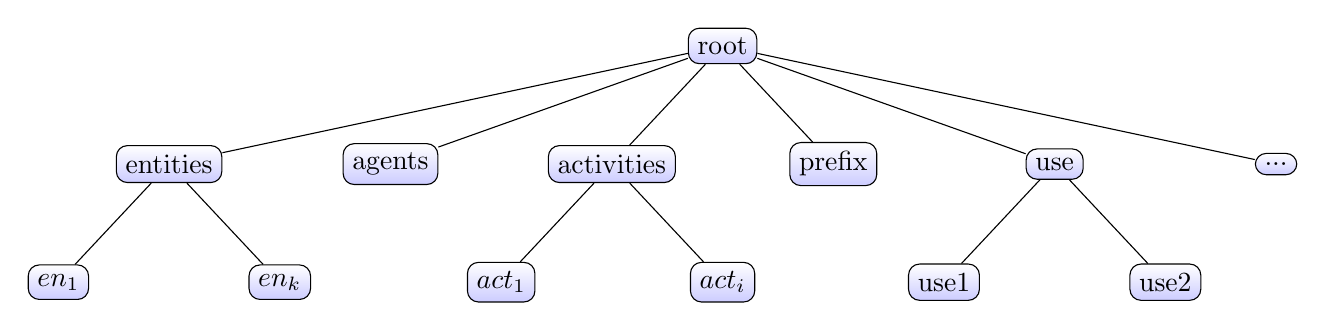
\begin{tikzpicture}[sibling distance=8em,
  every node/.style = {shape=rectangle, rounded corners,
    draw, align=center,
    top color=white, bottom color=blue!20}]]
  \node {root}
    child { node {entities}
         child { node {$en_1$} }
         child { node {$en_k$} }
     }
      child { node {agents} }
    child { node {activities}
      child { node {$act_1$} }
        child { node {$act_i$} }
        }
        child { node {prefix} }
        child { node {use}
        child { node {use1} }
        child { node {use2} }
        }
           child { node {...} }
        ;
\end{tikzpicture}
}
\end{center}
\end{minipage}
\caption{Top-key level of a PROV-JSON trace}
\label{prov-json-skeleton}
\end{figure}



The provenance traces represented in PROV-JSON format generally form a graph, that we define as follows. 

\begin{definition}[Provenance graph]
\label{def:prov-graph}
A provenance graph is a directed graph $G_P(V, R)$, where $V$ is the set of vertices and $R$ maps to provenance relationships.
Let $root \subseteq V$ be a set of vertices with an in-degree of 0 and an out-degree larger than 0. These nodes represent entities that are derived as described by the provenance trace. Successors of $root$ are entities $En \subseteq V$, activities $Act \subseteq V$, and agents $Ag \subseteq V$ involved in generating the entities described by $root$.
Each edge $e = (\langle v_{1},v_{2} \rangle,t)$, represents a provenance relation $r \subseteq R$ of type $t$ (e.g. gen, use) between $v_{1}$ and $v_{2}$  where   $\{v_{1},v_{2}\} \subseteq V$.
\end{definition}


    Figure~\ref{fig:universityX} depicts an example of a provenance graph.
     %obtained  {\color{Fuchsia} when exploring data warehouses using \prototype{}, the instance of our visual data exploration framework \framework{}.
%    It describes the why-provenance of the result ranking of ``MIT'', that is, it returns the source data relevant to produce this result.
%    The set  $root$ contains a unique entity ``entity1'' that results from the ranking query.
%    This latter is presented as an activity that uses the entity ``entity0'' to generate the result. 
%    Figure~\ref{fig:universityX} further includes white boxes associated with each node in the provenance graph. These contain the concrete provenance information recorded for each node. For instance, the provenance recorded about ``entity1'' includes the name of the university and the ranking value.
    It describes the set of explorations steps (cf.~Definition~\ref{def:expo-step}, Page~\pageref{def:expo-step}) investigated  by the user. The set  $root$ contains the entity ``entity2'' (corresponding to the last reached exploration step )  and  the agent ``agent1'' (corresponding to the user). Figure~\ref{fig:universityX} further includes white boxes associated with each node in the provenance graph. These contain the concrete provenance information recorded for each node. For instance, the provenance recorded about ``entity2'' includes the ids of the query and the visualization inspected by the users.

\smallskip


\noindent \textbf{Structure-based provenance summarization. } The set of provenance graphs defined above serve as input to our structure-based provenance summary approach, which consists of two steps. First, we infer individual provenance structures associated to individual provenance traces (local structures inference in Figure~\ref{fig:overview}). The second step aggregates individual structures into a single W3C-PROV compliant graph that structurally summarizes input provenance traces. 
More formally, we define the structure-based summary graph as follows.


\begin{definition}[Structure-based summary graph]A structure-based summary graph is a W3C-PROV compliant directed graph $SSG(PS_s, RS_s)$ associated to a set of provenance graphs $G$=\{$G_{P1}, \ldots,G_{Pn}$\} where $PS_s$ is the set of vertices referring to provenance structures defined later in Definition~\ref{def:prov-type} and $RS_s$ are edges mapping to the set of inferred provenance relationships. %\mel{Re reviewer 1: maybe ref to inference rules?)} 
Each relation $r \subseteq RS_s$ is presented as $ (\langle ps_{1},ps_{2}\rangle,t,c)$ where  $\langle ps_{1},ps_{2}\rangle$ is the edge connecting two structures $ps_1, ps_2 \in PS_s$, the type $t$ presents the provenance relationship type, and the cardinality $c$ is the number of provenance relationships in $G$, that follow the structure of $r$.
%quantifies the coverage of $r$ in $G$. 
\end{definition}


Figure~\ref{fig:Inf-type-university} shows an example of a structure-based summary graph. % inferred using our approach from provenance traces discussed in our illustrative Example~\ref{par:example}.
The content of this graph is discussed in Example~\ref{par:example2}.





\noindent \textbf{Visualization and analysis.} %To support users for different kinds of analysis over the structure-based summary graph, the last component of our pipeline provides different visualizations thereof.
The last component of our pipeline generates visualizations suited for various visual analysis tasks that rely on the structure-based summary graph. 
%{\color{Fuchsia}In contrast to previous steps depicted in Figure~\ref{fig:overview} that implement the \emph{provenance engine} module of our framework \framework{},  the visualization and analysis step describes possible techniques that can be used to implement the \emph{data display} module present also in the architecture of our framework \framework{} (cf.~Figure~\ref{fig:archi-FW}).}



\smallskip
%After this overview of the individual components of our solution, we now delve into the details of the structure-based provenance summarization component (Figure~\ref{sec:system}) and the visualization component (Figure~\ref{sec:vis}).
After this overview, we now delve into the details of individual components of our solution in Section~\ref{sec:system} and Section~\ref{sec:vis}.

